\chapter{Architecture}

\section{Block diagram}
The architecture for the full IP core is shown in the Figure~\ref{blockdiagram}. It consists of 2 major parts, the actual
exponentiation core (\verb|mod_sim_exp_core| entity) with a bus interface wrapped around it. In the following sections these 
different blocks are described in detail. The bus interface and the exponentiation core can run on different clock
frequencies, so they are independent of each other.\\
\begin{figure}[H]
\centering
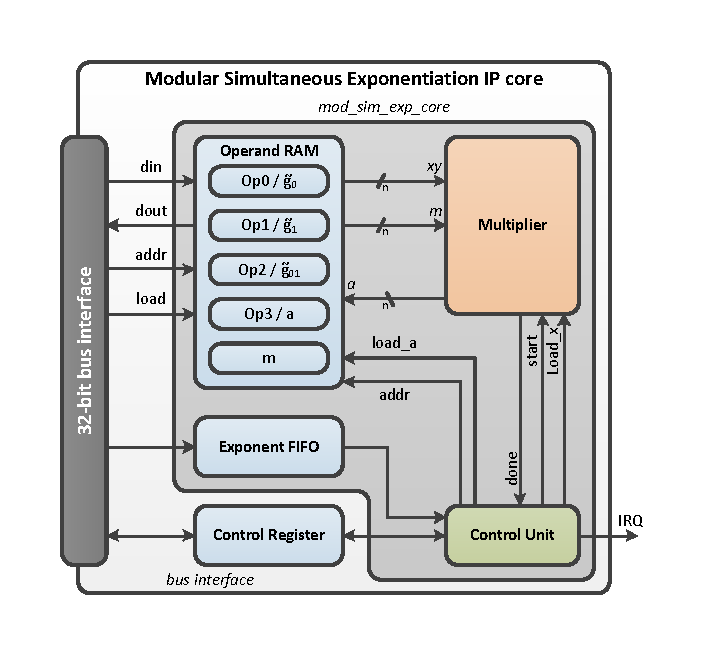
\includegraphics[trim=1.2cm 1.2cm 1.2cm 1.2cm, width=10cm]{pictures/block_diagram.pdf}
\caption{Block diagram of the Modular Simultaneous Exponentiation IP core}
\label{blockdiagram}
\end{figure}
\newpage

\section{Exponentiation core}
The exponentiation core (\verb|mod_sim_exp_core| entity) is the top level of the modular simultaneous exponentiation
core. It is made up by 4 main blocks (Figure~\ref{msec_structure}):\\

\begin{itemize}
	\item a pipelined Montgomery multiplier as the main processing unit
	\item RAM to store the operands and the modulus
	\item a FIFO to store the exponents
	\item a control unit which controls the multiplier for the exponentiation and multiplication operations
\end{itemize}

\begin{figure}[H]
\centering
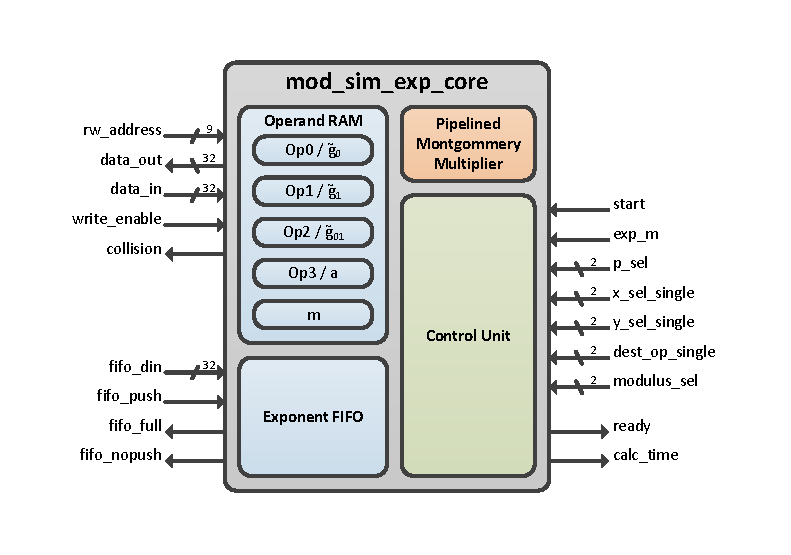
\includegraphics[trim=1.2cm 1.2cm 1.2cm 1.2cm, width=10cm]{pictures/mod_sim_exp_core.pdf}
\cprotect\caption{\verb|mod_sim_exp_core| structure}
\label{msec_structure}
\end{figure}

The multiplier and control unit operate on the \verb|core_clk| clock frequency and the interface to the operand RAM and
exponent FIFO operates on the \verb|bus_clk| clock frequency. The transition between the 2 clock domains is mainly
implemented by the RAM and FIFO. For the remainder, the necessary control signals are synchronised to the
\verb|bus_clk|. Thus when using the \verb|mod_sim_exp_core|, one can thus assume that al ports are operating on the
\verb|bus_clk| clock signal.

\subsection{Multiplier}
The kernel of this design is a pipelined Montgomery multiplier. A Montgomery multiplication\cite{MontModMul} allows efficient implementation of a
modular multiplication without explicitly carrying out the classical modular reduction step. Right-shift operations ensure that the length of the (intermediate) results does not exceed $n+1$ bits. The result of a Montgomery multiplication is given by~(\ref{eq:mont}):
\begin{align}\label{eq:mont}
r = x \cdot y \cdot R^{-1} \bmod m \hspace{1.5cm}\text{with } R = 2^{n}
\end{align}
For the structure of the multiplier, the work of \textit{Nedjah and Mourelle}\cite{NedMour} is used as a basis. They show that for large operands ($>$512 bits) the $time\times area$ product is minimal when a systolic implementation is used. This construction is composed of cells that each compute a bit of the (intermediate) result.

Because a fully unrolled two-dimensional systolic implementation would require too many resources, a systolic array (one-dimensional) implementation is chosen. This implies that the intermediate results are fed back to the same same array of cells through a register. A shift register will shift-in a bit of the $x$ operand for every step in the calculation (figure~\ref{mult_structure}). When multiplication is completed, a final check is made to ensure the result is smaller than the modulus. If not, a final reduction with $m$ is necessary.

\textbf{Note:} For this implementation the modulus $m$ has to be uneven to obtain a correct result. However, we can assume that for cryptographic applications, this is the case.


\begin{figure}[H] 
\centering 
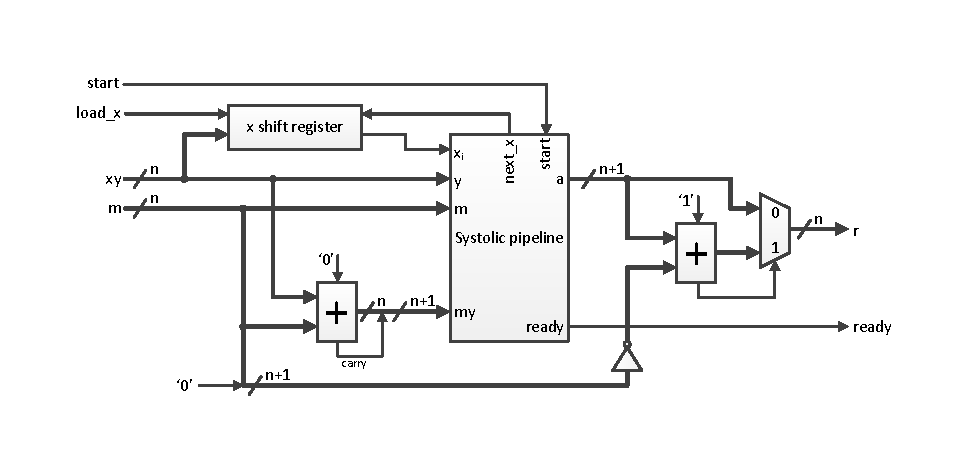
\includegraphics[trim=1.2cm 1.2cm 1.2cm 1.2cm, width=15cm]{pictures/mult_structure.pdf}
\caption{Multiplier structure. For clarification the $my$ adder and reduction logic are depicted separately, whereas in practice they are internal parts of the stages. (See Figure~\ref{stage_structure})}
\label{mult_structure}
\end{figure}

\subsubsection{Stage and pipeline structure}
The Montgomery algorithm uses a series of additions and right shifts to obtain the desired result. The main disadvantage
is the carry propagation in the adder, and therefore a pipelined version is used. The length of the operands ($n$) and
the number of pipeline stages can be chosen before synthesis. The user has the option to split the pipeline into 2
smaller parts so there are 3 operand lengths available during runtime\footnote{e.g. a total pipeline length of 1536 bit
split into a part of 512 bit and a part of 1024 bit}.

The stages and first and last cell logic design are presented in Figure~\ref{stage_structure}. Each stage takes in a
part of the modulus $m$ and $y$ operand and for each step of the multiplication, a bit of the $x$ operand is fed to the
pipeline (together with the generated $q$ signal), starting with the Least Significant Bit. The systolic array cells
need the modulus $m$, the operand $y$ and the sum $m+y$ as an input. The result from the cells is latched into a
register, and then passed back to the systolic cells for the next bit of $x$. During this pass the right shift operation
is implemented. Each stage thus needs the least significant bit from the next stage to calculate the next step. Final
reduction logic is also present in the stages for when the multiplication is complete.

An example of the standard pipeline structure is presented in Figure~\ref{pipeline_structure}. It is constructed using
stages with a predefined width. The first cell logic processes the first bit of the $m$ and $y$ operand and generates
the $q$ signal. The last cell logic finishes the reduction and selects the correct result. For operation of this
pipeline, it is clear that each stage can only compute a step every 2 clock cycles. This is because the stages rely on
the result of the next stage.

In Figure~\ref{pipeline_structure_split} an example pipeline design is drawn for a split pipeline. All multiplexers on
this figure are controlled by the pipeline select signal (\verb|p_sel|). During runtime the user can choose which part
of the pipeline is used, the lower or higher part or the full pipeline.

\newpage 
\begin{figure}[H]
\centering
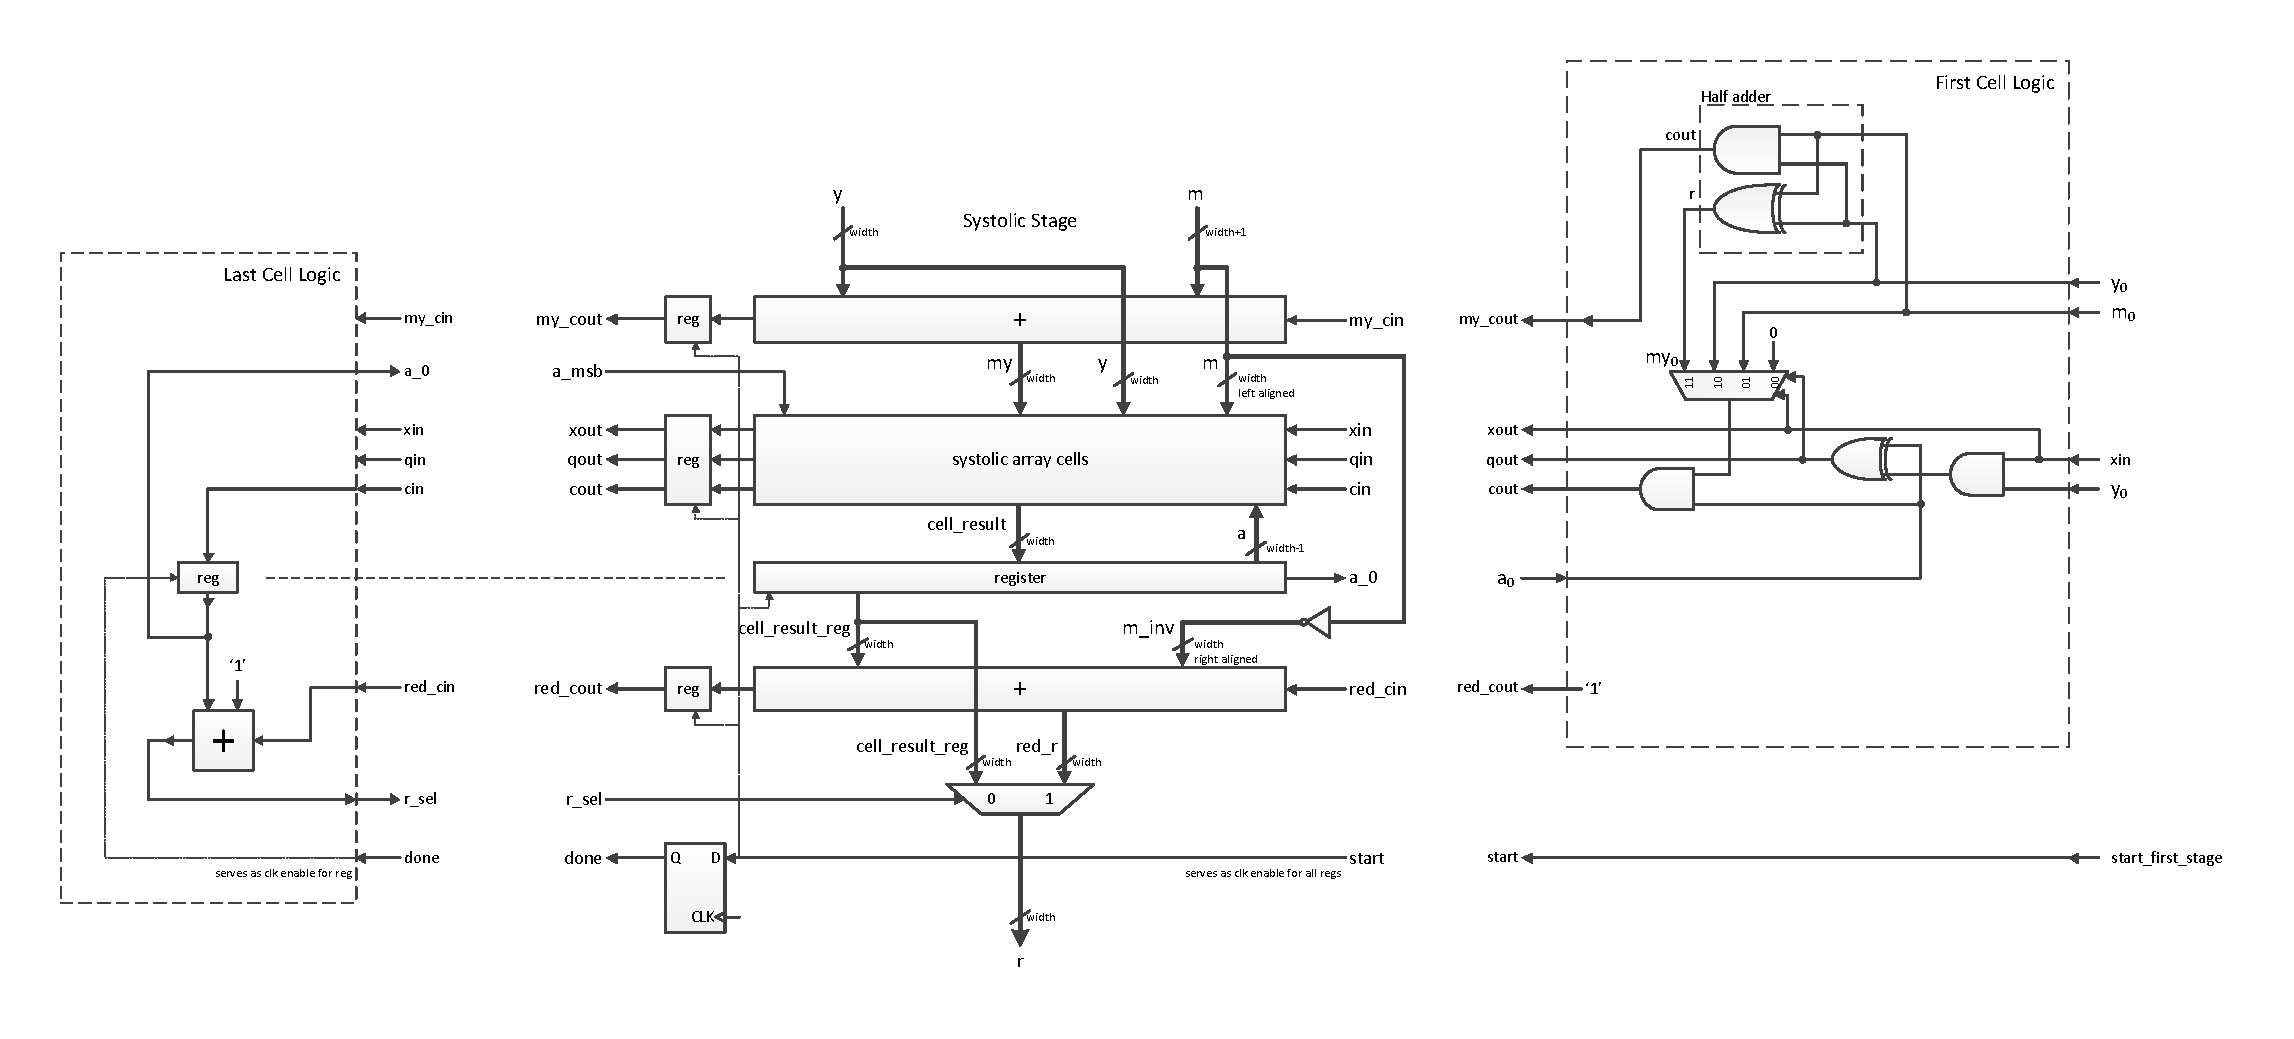
\includegraphics[trim=1.2cm 1.2cm 1.2cm 1.2cm, width=25cm, angle=90]{pictures/sys_stage.pdf}
\caption{Pipeline stage and first and last cell logic}
\label{stage_structure}
\end{figure}
\newpage

\newpage 
\begin{figure}[H]
\centering
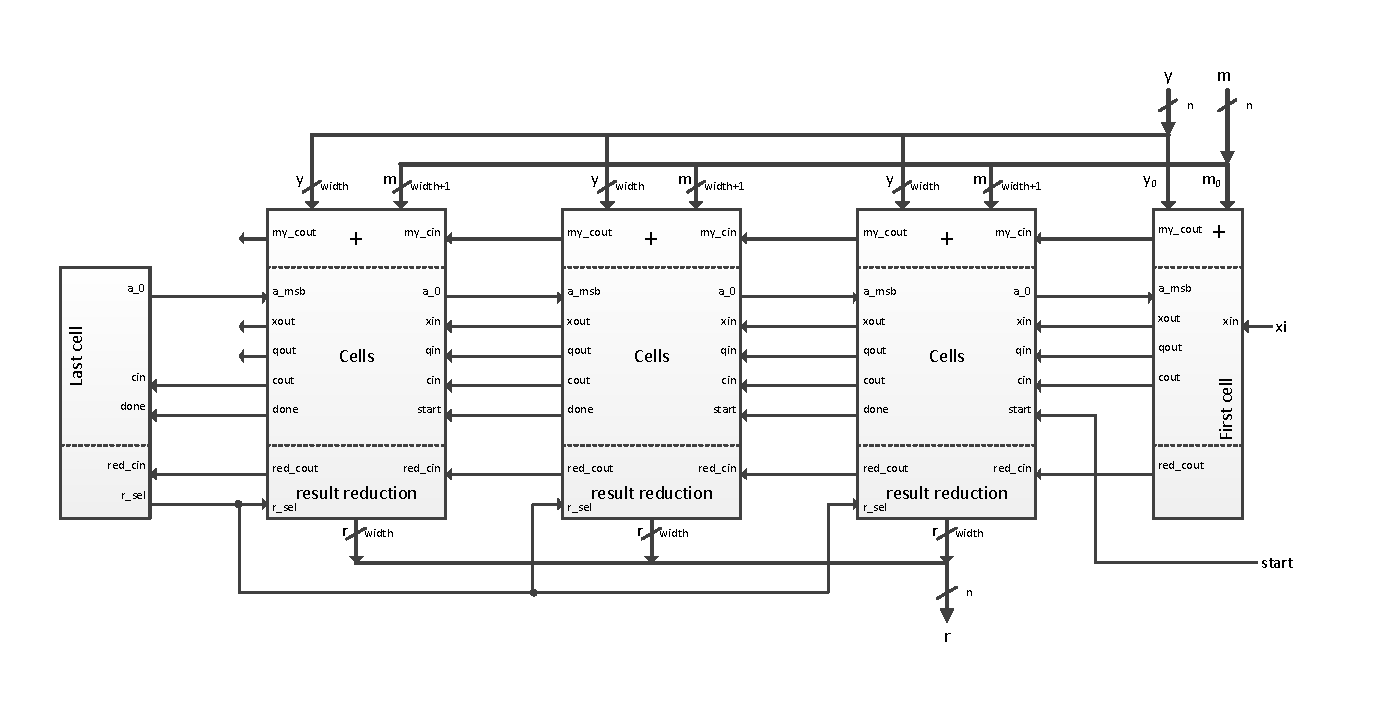
\includegraphics[trim=1.2cm 1.2cm 1.2cm 1.2cm, width=25cm, angle=90]{pictures/sys_pipeline_notsplit.pdf}
\caption{Example of the pipeline structure (3 stages)}
\label{pipeline_structure}
\end{figure}
\newpage

\newpage 
\begin{figure}[H]
\centering
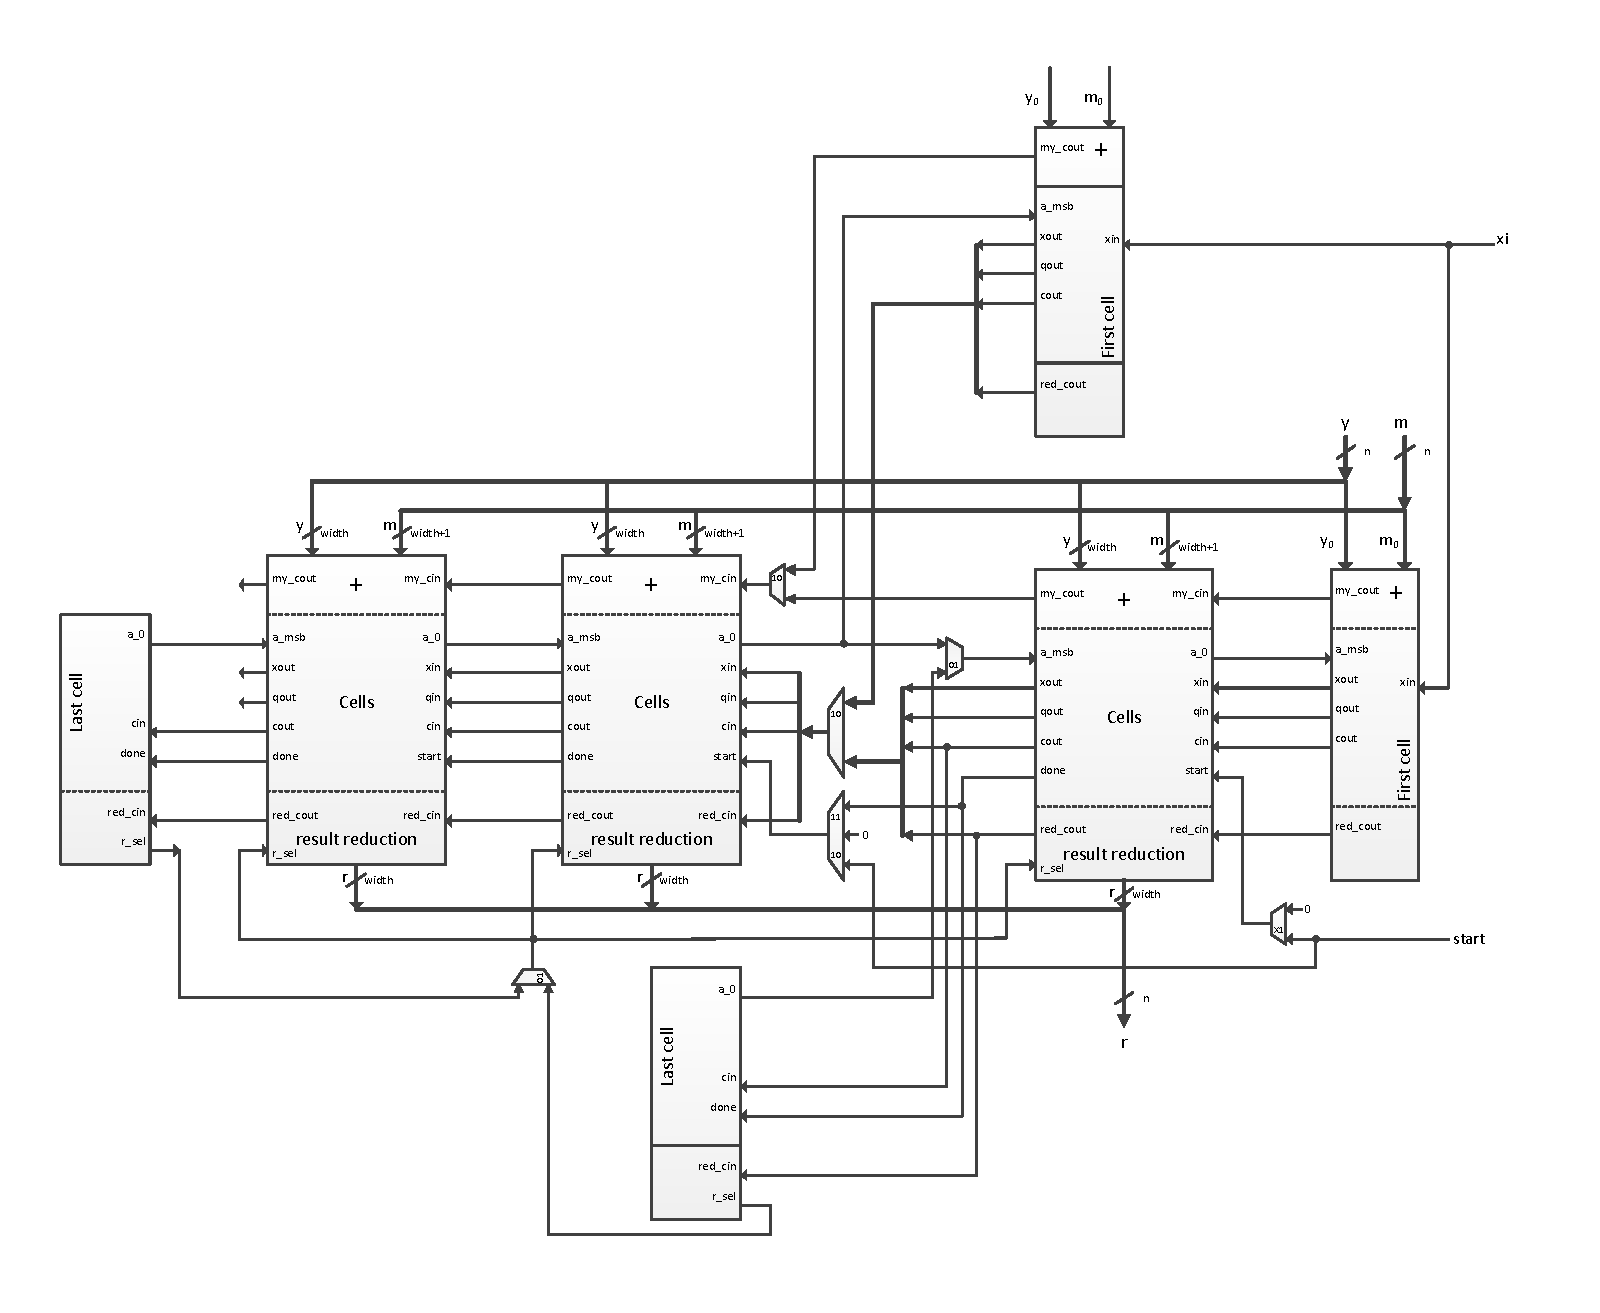
\includegraphics[trim=1.2cm 1.2cm 1.2cm 1.2cm, width=22cm, angle=90]{pictures/sys_pipeline.pdf}
\caption{Example of a split pipeline (1+2 stages)}
\label{pipeline_structure_split}
\end{figure}
\newpage


\subsection{Operand RAM and exponent FIFO} \label{subsec:RAM_and_FIFO}
The core's RAM is designed to store 4 operands and a modulus. \footnote{This is the default configuration. The number of operands can be increased, but the control logic is only designed to work with the default configuration.} Three (3) options are available for the implementation of the RAM. Setting the parameter \verb|C_MEM_STYLE|, will change the implementation style. All styles try to use the RAM resources available on the FPGA.

If the FPGA supports asymmetric RAMs, i.e. with a different read and write width, we suggest that the option \verb|"asym"| is selected. Since the (device specific) RAM blocks are inferred through code, it is imperative to select the right device (\verb|C_FPGA_MAN|), as this inference is different between manufacturers. Currently, only Altera and Xilinx are supported.

If there's no asymmetric RAM support, the option \verb|"generic"| should be selected. This option will work for most FPGAs, but the disadvantage is that it will use more resources than the \verb|"asym"| option. This is because a significant number of LUTs will be used to construct an asymmetric RAM.

For both options the size of the RAM adapts dynamically to the chosen pipeline width (\verb|C_NR_BITS_TOTAL|).

Finally, the option \verb|"xil_prim"| is targeted specifically to Xilinx devices. It uses blocks of RAM generated with CoreGen. These blocks are of a fixed width and this results in a fixed RAM of 4x1536 bit for the operands and 1536 bit for the modulus. This option is deprecated in favor of \verb|"asym"|.

Reading and writing (from the bus side) to the operands and modulus is done one 32-bit word at a time. If using a split pipeline, it is important that operands for the higher part of the pipeline are loaded into the RAM with preceding zero's for the lower bits of the pipeline. As a rule of thumb, the number of FPGA RAM blocks that will be used is given by (\ref{eq:ramblocks}):
\begin{align}
	2 \cdot \mathtt{C\_NR\_BITS\_TOTAL} / 32\label{eq:ramblocks}
\end{align}
\newline

To store the exponents, there is a FIFO of 32 bit wide. Every 32 bit entry has to be formatted as 16 bit of $e_0$ for the
lower part [15:0] and 16 bit of $e_1$ for the higher part [31:16]. Entries have to be pushed in the FIFO starting with the least significant word and ending with the most significant word of the exponents.

For the FIFO there are 2 styles available. The implementation style depends on the style of the operand memory and it can not be set directly. When the RAM option \verb|"xil_prim"| is chosen, the resulting FIFO will use the FIFO18E1 primitive. It is able to store 512 entries, meaning 2 exponents of each 8192 bit long.

When the RAM options \verb|"generic"| or \verb|"asym"| are chosen, a generic FIFO \footnote{This FIFO is a slightly
modified version of the generic FIFOs project at OpenCores.org (http://opencores.org/project,generic\_fifos).} will be
implemented.
This consist of a dual port symmetric RAM with the control logic for a FIFO. The depth of this generic FIFO is adjustable with the parameter \verb|C_FIFO_AW|. The number of RAM blocks for the FIFO is given by (\ref{eq:fifoblocks}), where
\verb|RAMBLOCK_SIZE| is the size [bits] of the FPGA's RAM primitive.
\begin{align}
	\left[\left(\mathtt{2^{C\_FIFO\_AW}}+1\right) \cdot 32 \right]/ \mathtt{RAMBLOCK\_SIZE} \label{eq:fifoblocks}
\end{align}

\subsection{Control unit}
The control unit loads in the operands and has full control over the multiplier. For single multiplications, it latches in 
the $x$ operand, then places the $y$ operand on the bus and starts the multiplier. In case of an exponentiation, the FIFO is 
emptied while the necessary single multiplications are performed. When the computation is done, the ready signal is 
asserted to notify the system.

\newpage
\subsection{IO ports and memory map}
The \verb|mod_sim_exp_core| IO ports\\
\newline
% Table generated by Excel2LaTeX
\begin{tabular}{|l|c|c|p{8cm}|}
\hline
\rowcolor{Gray}
\textbf{Port} & \textbf{Width} & \textbf{Direction} & \textbf{Description} \bigstrut\\
\hline
\verb|core_clk|   & 1     & in    & core clock input, clock signal for the multiplier and control unit \bigstrut\\
\hline
\verb|bus_clk|   & 1     & in    & bus clock input, clock signal for all core IO \bigstrut\\
\hline
\verb|reset| & 1     & in    & reset signal (active high) resets the pipeline, fifo and control logic \bigstrut\\
\hline
\multicolumn{4}{|l|}{\textbf{\textit{operand memory interface}}} \bigstrut\\
\hline
\verb|rw_address| & 9     & in    & operand memory read/write address (structure descibed below) \bigstrut\\
\hline
\verb|data_out| & 32    & out   & operand data out (0 is lsb) \bigstrut\\
\hline
\verb|data_in| & 32    & in    & operand data in (0 is lsb) \bigstrut\\
\hline
\verb|write_enable| & 1     & in    & write enable signal, latches \verb|data_in| to operand RAM \bigstrut\\
\hline
\verb|collision| & 1     & out   & collision output, asserts on a write error \bigstrut\\
\hline
\multicolumn{4}{|l|}{\textbf{\textit{exponent FIFO interface}}} \bigstrut\\
\hline
\verb|fifo_din| & 32    & in    & FIFO data in, bits [31:16] for $e_1$ operand and bits [15:0] for $e_0$ operand \bigstrut\\
\hline
\verb|fifo_push| & 1     & in    & push \verb|fifo_din| into the FIFO \bigstrut\\
\hline
\verb|fifo_nopush| & 1     & out   & flag to indicate if there was an error pushing the word to the FIFO \bigstrut\\
\hline
\verb|fifo_full| & 1     & out   & flag to indicate the FIFO is full \bigstrut\\
\hline
\multicolumn{4}{|l|}{\textbf{\textit{control signals}}} \bigstrut\\
\hline
\verb|x_sel_single| & 2     & in    & selection for x operand source during single multiplication \bigstrut\\
\hline
\verb|y_sel_single| & 2     & in    & selection for y operand source during single multiplication \bigstrut\\
\hline
\verb|dest_op_single| & 2     & in    & selection for the result destination operand for single multiplication \bigstrut\\
\hline
\verb|p_sel| & 2     & in    & specifies which pipeline part to use for exponentiation / multiplication. \bigstrut[t]\\
      &       &       & ``01'' : use lower pipeline part \\
      &       &       & ``10'' : use higher pipeline part \\
      &       &       & ``11'' : use full pipeline \bigstrut[b]\\
\hline
\verb|modulus_sel| & 1     & in    & selection for which modulus to use for the calculations (only available if \verb|C_MEM_STYLE| = \verb|"generic"| or \verb|"asym"|). Otherwise set to 0 \bigstrut\\
\hline
\verb|exp_m| & 1     & in    & core operation mode. ``0'' for single multiplications and ``1'' for exponentiations \bigstrut\\
\hline
\verb|start| & 1     & in    & start the calculation for current mode \bigstrut\\
\hline
\verb|ready| & 1     & out   & indicates the multiplication/exponentiation is done \bigstrut\\
\hline
\verb|calc_time| & 1     & out   & is high during a multiplication, indicator for used calculation time \bigstrut\\
\hline
\end{tabular}%
\newpage
The \verb|mod_sim_exp_core| parameters\\
\begin{center}
	\begin{tabular}{|l|p{6.5cm}|c|l|}
		\hline
		\rowcolor{Gray}
		\textbf{Name} & \textbf{Description} & \textbf{VHDL Type} &\textbf{Default Value} \bigstrut\\
		\hline
		\verb|C_NR_BITS_TOTAL| & total width of the multiplier in bits & integer & 1536\bigstrut\\
		\hline
		\verb|C_NR_STAGES_TOTAL| & total number of stages in the pipeline & integer & 96\bigstrut\\
		\hline
		\verb|C_NR_STAGES_LOW| & number of lower stages in the pipeline, defines the bit-width of the lower pipeline part & integer & 32 \bigstrut\\
		\hline
		\verb|C_SPLIT_PIPELINE| & option to split the pipeline in 2 parts & boolean & true \bigstrut\\
		\hline
		\verb|C_FIFO_AW| & address width of the generic FIFO pointers, FIFO size is equal to $2^{C\_FIFO\_AW} $. & integer & 7 \bigstrut\\
						 & only	applicable if \verb|C_MEM_STYLE| = \verb|"generic"| or \verb|"asym"|  & & \\
		\hline
		\verb|C_MEM_STYLE| & select the RAM memory style (3 options): & string & \verb|"generic"| \bigstrut\\
							& \verb|"generic"| : use general 32-bit RAMs & & \\
      						& \verb|"asym"| : use asymmetric RAMs & & \\
      						& (For more information see \ref{subsec:RAM_and_FIFO}) & & \\
      						& \verb|"xil_prim"| : use xilinx primitives & &\\
      						& (deprecated) & & \bigstrut[b] \\
		\hline
		\verb|C_FPGA_MAN| & device manufacturer: & & \\
						& \verb|"xilinx"| or \verb|"altera"| & string & \verb|"xilinx"| \bigstrut\\
		\hline
	\end{tabular}%
\end{center}

The following figure describes the structure of the Operand RAM memory, for every operand there is a space of 2048 bits 
reserved. So operand widths up to 2048 bits are supported.\\
\newline \\
\begin{figure}[H]
\centering
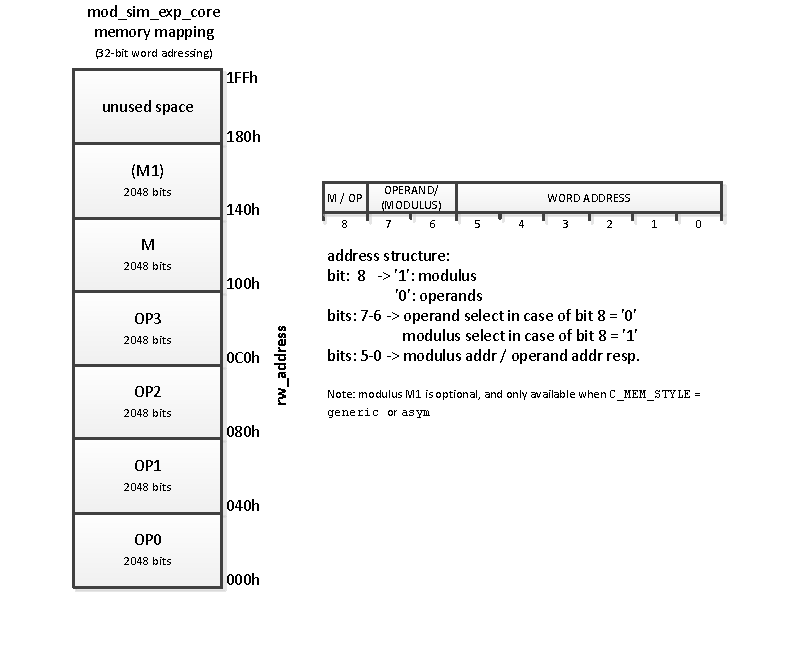
\includegraphics[trim=1.2cm 1.2cm 1.2cm 1.2cm, width=15cm]{pictures/msec_memory.pdf}
\caption{Address structure of the exponentiation core}
\label{Address_structure}
\end{figure}

\section{Bus interface}
The bus interface implements the register necessary for the control unit inputs to the \verb|mod_sim_exp_core| entity.
It also maps the memory to the required bus and connects the interrupt signals. The embedded processor then has full control
over the core.